%!TEX root = ../thesis.tex
\newchap{The CMS experiment at LHC}\label{sec:CMS}
\vspace{-1cm}
\minitoc

CERN is the largest international particle physics research center in the world. It is located across the Franco-Swiss border in Meyrin, near Geneva, and was founded in 1954, after the end of World War II, by twelve European countries.\\
Today, more than 100 countries, 500 institutes, and 13000 users collaborate to the CERN activities.

\section{The Large Hadron Collider}
The CERN's major facility is the Large Hadron Collider (LHC), a proton-proton (pp) and ions collider that, with its lengths of 26.7 km and its energy in the center of mass of $\sqrt{s}=13.6\TeV$, is the largest and the most powerful particle accelerator ever built in the world.\\
As shown in \Fig{fig:cern}, the LHC is just the last stage of a chain of accelerators. The protons obtained from ionizing hydrogen are grouped in bunches through a quadrupole magnet and then are sent to a chain of accelerators that increase progressively the energy of the protons.
Before entering the LHC, the proton beam is split into two beam lines that travel in opposite directions and then are accelerated by radiofrequency (RF) cavities that are tuned to oscillate at 400MHz. In addition to RF cavities, quadrupoles are used to keep the beam focused and dipoles to bend the beam \cite{Bruning2004LHCReport}.\\
Once the beam is stabilized, the proton bunches collide in four different points where the experiments ATLAS, CMS, LHCb, and ALICE are located.\\
ATLAS (A Toroidal LHC ApparatuS) and CMS (Compact Muon Solenoid) are general-purpose detectors and are the ones that in the 2012 discovered the Higgs boson  \cite{Chatrchyan2012ObservationLHC,Aad2012ObservationLHC}, LHCb (LHC beauty) is a forward detector designed to study the physics of the B mesons and the matter-antimatter asymmetry and ALICE (A Large Ion Collider Experiment) is a detector devoted to the study of quark-gluon plasma and extreme phases of QCD matter through the analysis of lead ion collisions.
\begin{figure}[h!]
    \centering
    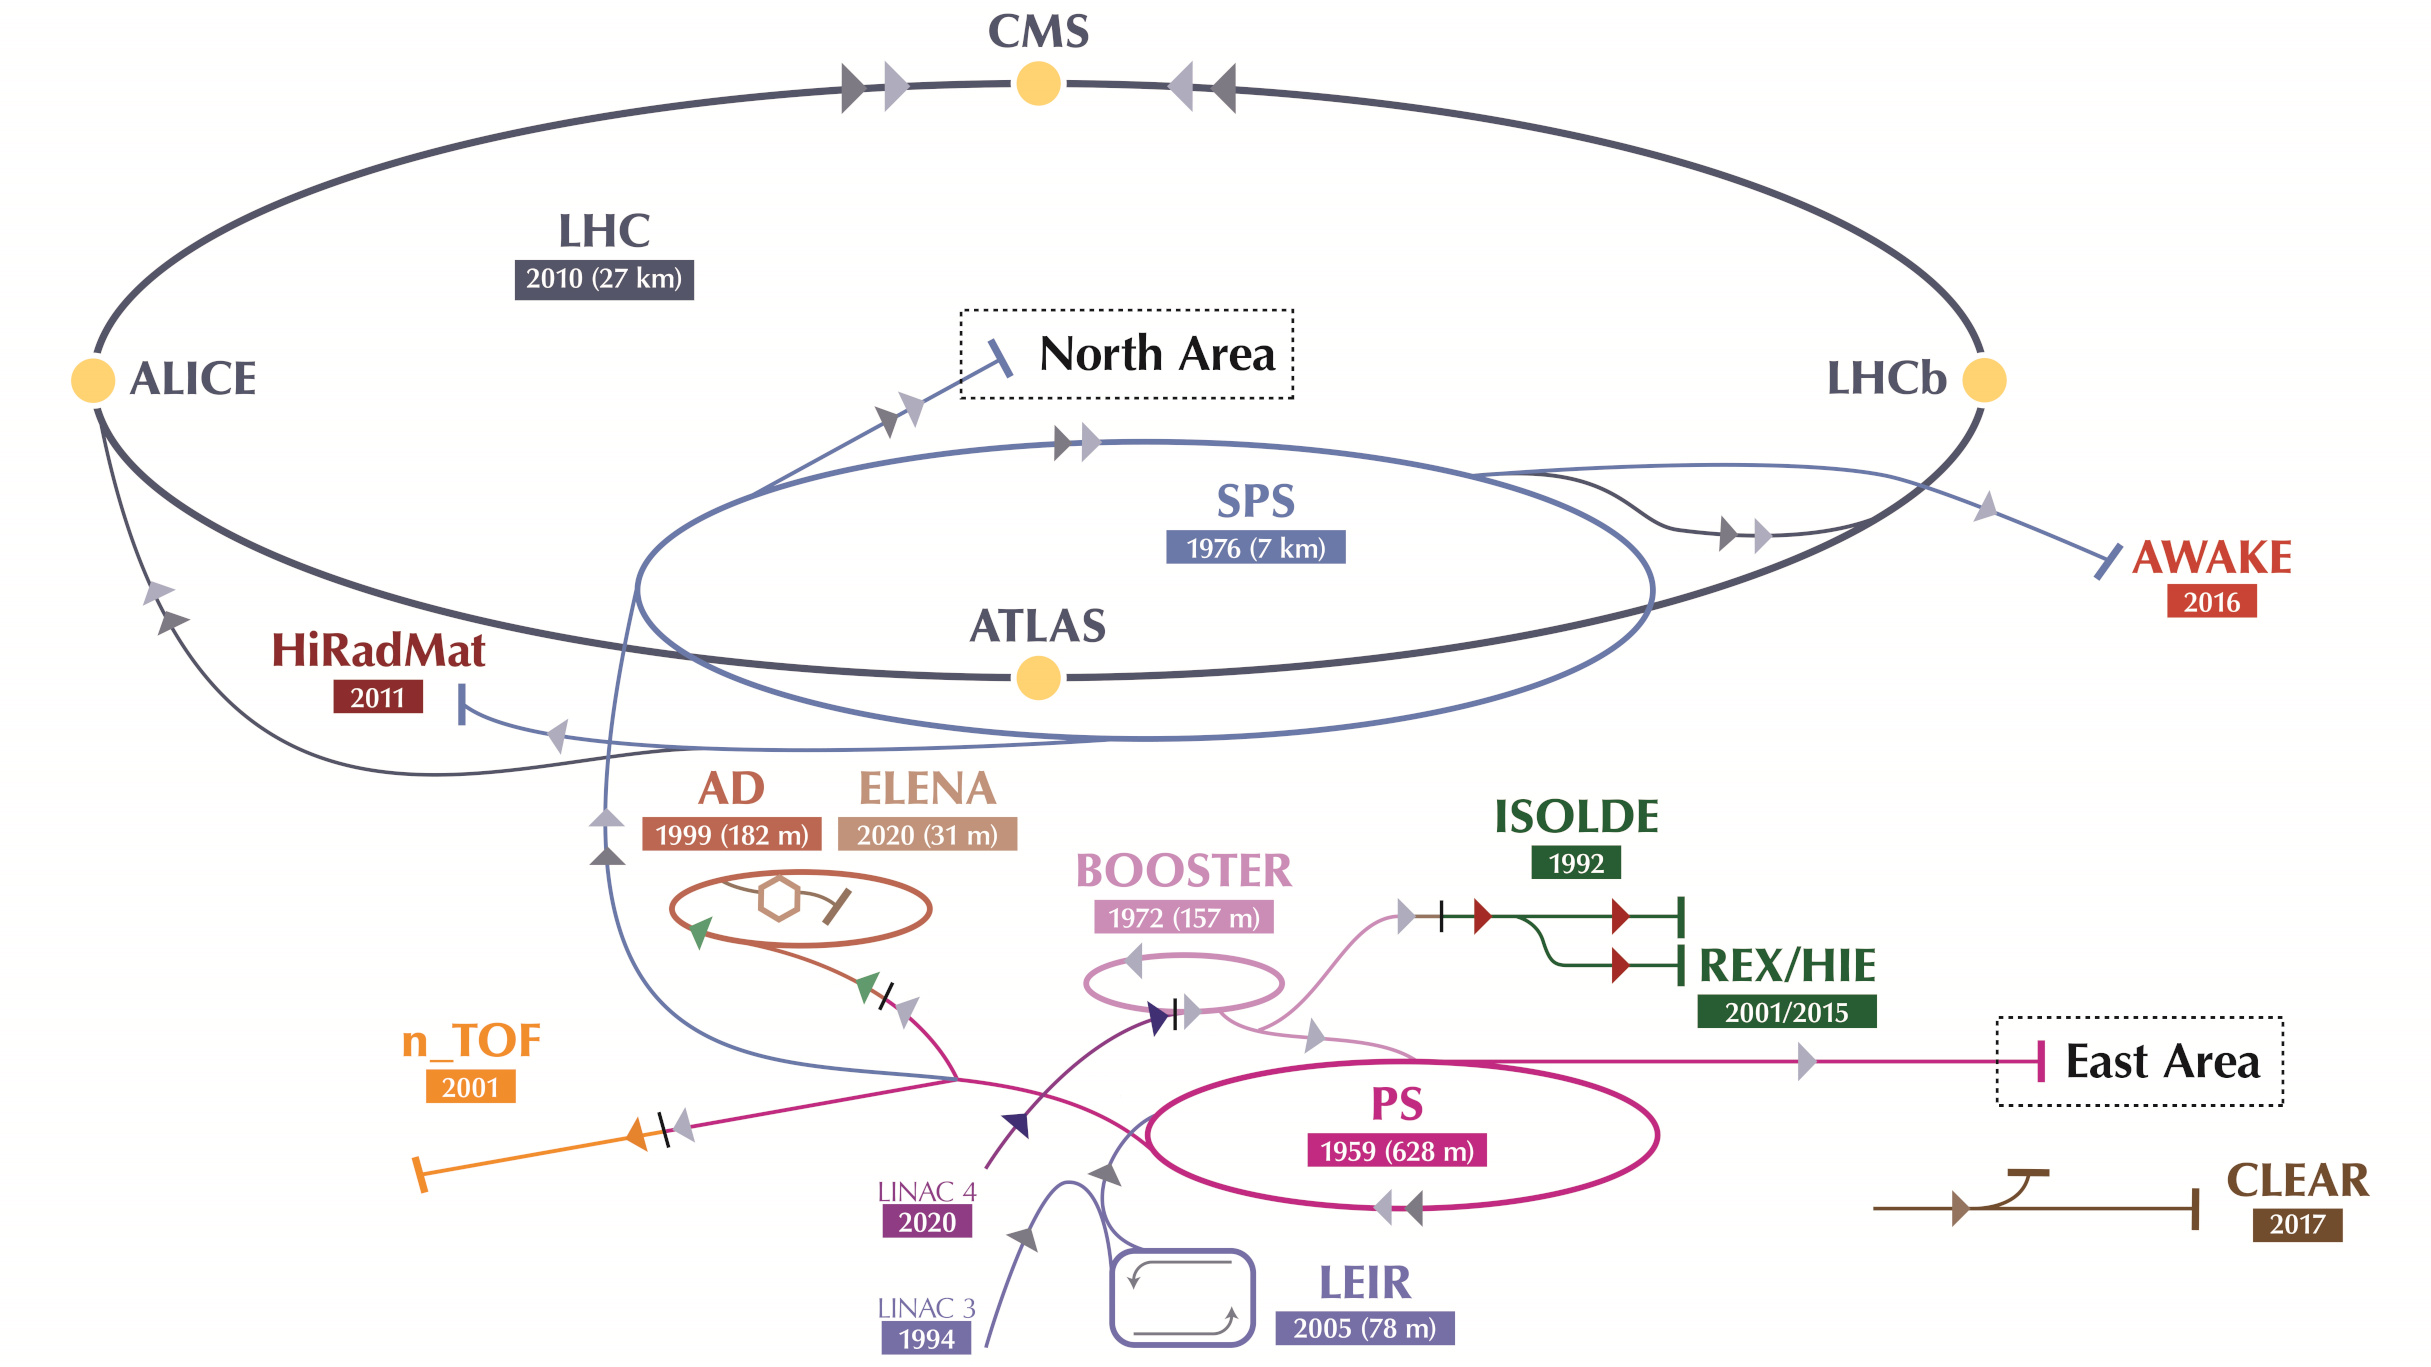
\includegraphics[width=\textwidth]{fig//chap03-cms/cern.jpg}
    \caption{CERN's accelerator complex. The accelerating chain is: LINAC2 (50 \MeV) $\to$ Booster (1.4\GeV) $\to$ Proton Synchrotron (PS) (26\GeV) $\to$ Super Proton Synchrotron (450\GeV) $\to$ LHC (13/14 \TeV). The intermediate accelerators also provide a proton beam to other smaller experiments and facilities. \cite{Panoramas}}
    \label{fig:cern}
\end{figure}

\paragraph*{Luminosity}
The \emph{instantaneous luminosity} is defined as the ratio between the event rate produced for a given process and its cross-section
\begin{equation}
    \mathcal{L} = \frac{\partial N}{\partial t} \frac{1}{\sigma} 
\end{equation}
and can be expressed also as a function of the beam parameters
\begin{equation}
    \mathcal{L}=\frac{N_{p}^{2}f\gamma_{r}}{4\pi\epsilon_{n}\beta\sp{\ast}}F\ 
\end{equation}
where $N_p$ is the number of protons per bunch, $f$ the bunch frequency, $\gamma_r$ the relativistic factor, and $\epsilon_n, \beta^*, F$ are geometrical factors that take into account the shape of the beam and the crossing angle between the two beams in the interaction point (IP).\\
These parameters depend on the so-called “filling scheme”, the chosen pattern of filled and empty bunch crossings used in a single fill.
A typical filling scheme is composed of long strings of consecutive bunches called a “train”, with the individual trains separated by gaps of varying lengths. Filling schemes also include some number of non-colliding bunch crossings that can be used to study effects from beam-induced background \cite{CMSCollaboration2021PrecisionCMS}.\\
The LHC was designed to achieve an instantaneous luminosity of $\mathcal{L}=10^{34} cm^{-2}s^{-1}$ but, in 2018, the LHC was able to reach a peak luminosity of $\mathcal{L}=2.1 \cdot 10^{34} cm^{-2}s^{-1}$ doubling the nominal design value. Increasing the luminosity is essential to observe rare events and to decrease the statistical uncertainties of every measurement, but it has a drawback: the number of simultaneous pp interactions, called pileup (PU), increases with the instantaneous luminosity, making the event reconstruction more difficult and generating underlying events, \ie the hadronic activity that does not originate from the hard scattering. PU effects can be mitigated thanks to high-granularity detectors and advanced reconstruction algorithms.\\
The amount of recorded data is quantified by the \emph{integrated luminosity}, the time integral of the instantaneous luminosity $\mathcal{L}_I=\int dt \mathcal{L}(t)$.


\begin{figure}[h!]
    \centering
    \begin{minipage}{0.52\linewidth}
        
        \centering
        \includegraphics[width=\linewidth]{fig//chap03-cms/lumi.png}
        (a)
    \end{minipage}
    \begin{minipage}{0.47\linewidth}
        \vspace{0.6cm}
        \centering
        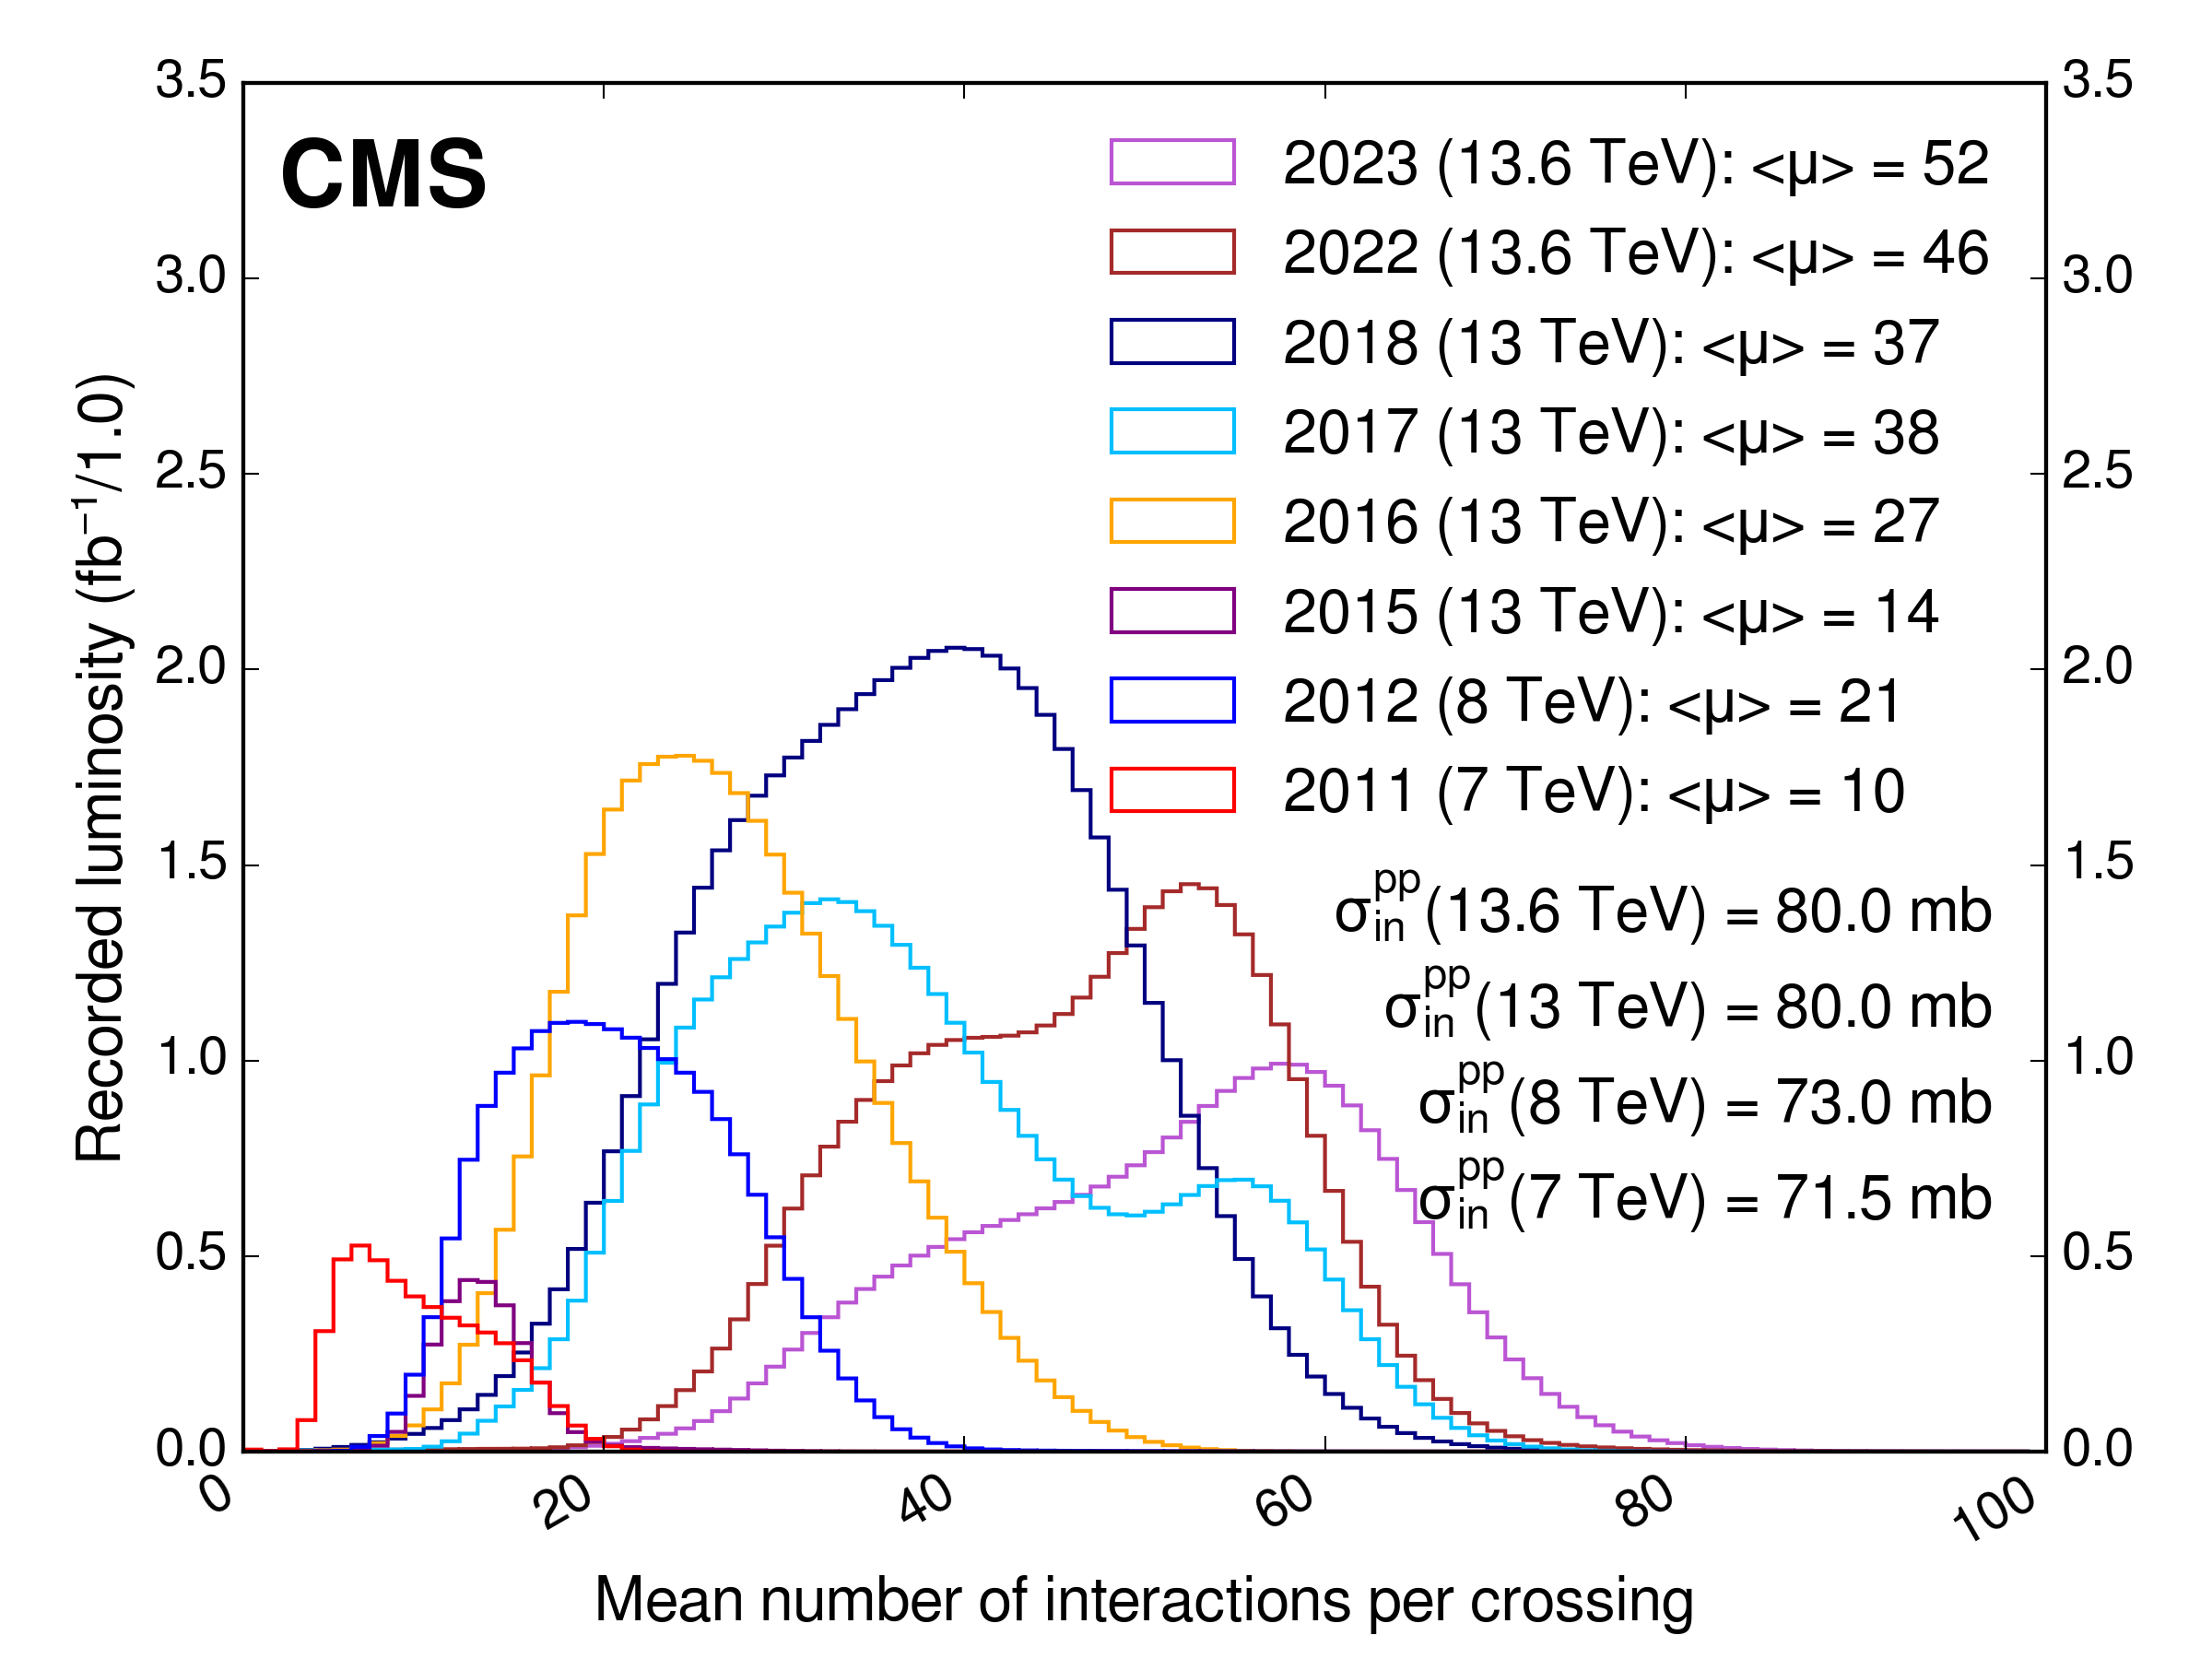
\includegraphics[width=\linewidth]{fig//chap03-cms/pileup.png}
        (b)
    \end{minipage}
    \caption{(a) cumulative integrated luminosity delivered and recorded by the CMS experiment; (b) PU distribution across different years at the CMS experiment \cite{LumiPublicResultsTWiki}}
    \label{fig:lumi_pu}
\end{figure}
\paragraph*{Physics runs}
The LHC program covers a period of $\sim$ 30 years, divided into two phases. 
The \emph{Phase I} includes Run I (2011-2012), Run II (2015-2018), and Run III (2022-2025).
During Phase I the center of mass energy was increased from $7 \TeV$ to $13.6 \TeV$ and the instantaneous luminosity reached a peak of $\mathcal{L}= 2.1 \cdot 10^{34}cm^{-2} s^{-1}$. \\
At the end of 2025, the LHC will enter the \emph{High Luminosity} LHC (HL-LHC) phase, a new phase of upgrades that will take the center of mass energy to 14 \TeV and to an instantaneous luminosity of $\mathcal{L}=5 \cdot 10^{34}cm^{-2} s^{-1}$, providing an integrated luminosity during all the Phase II (2029-2040) of $\mathcal{L}_I=3000 fb^{-1}$, ten times more than in Phase I.\\
During the long shutdown 3 (LS3: 2025-2029) the detectors will be upgraded, along the LHC, to be able to work in such a challenging environment that causes more radiation damage, especially in the forward subdetectors, and with a significant PU increase. up to <PU>$\sim 200$ \cite{Aberle2020SubmitterReport}. 

\iffalse
\begin{figure}[h!]
    \centering
    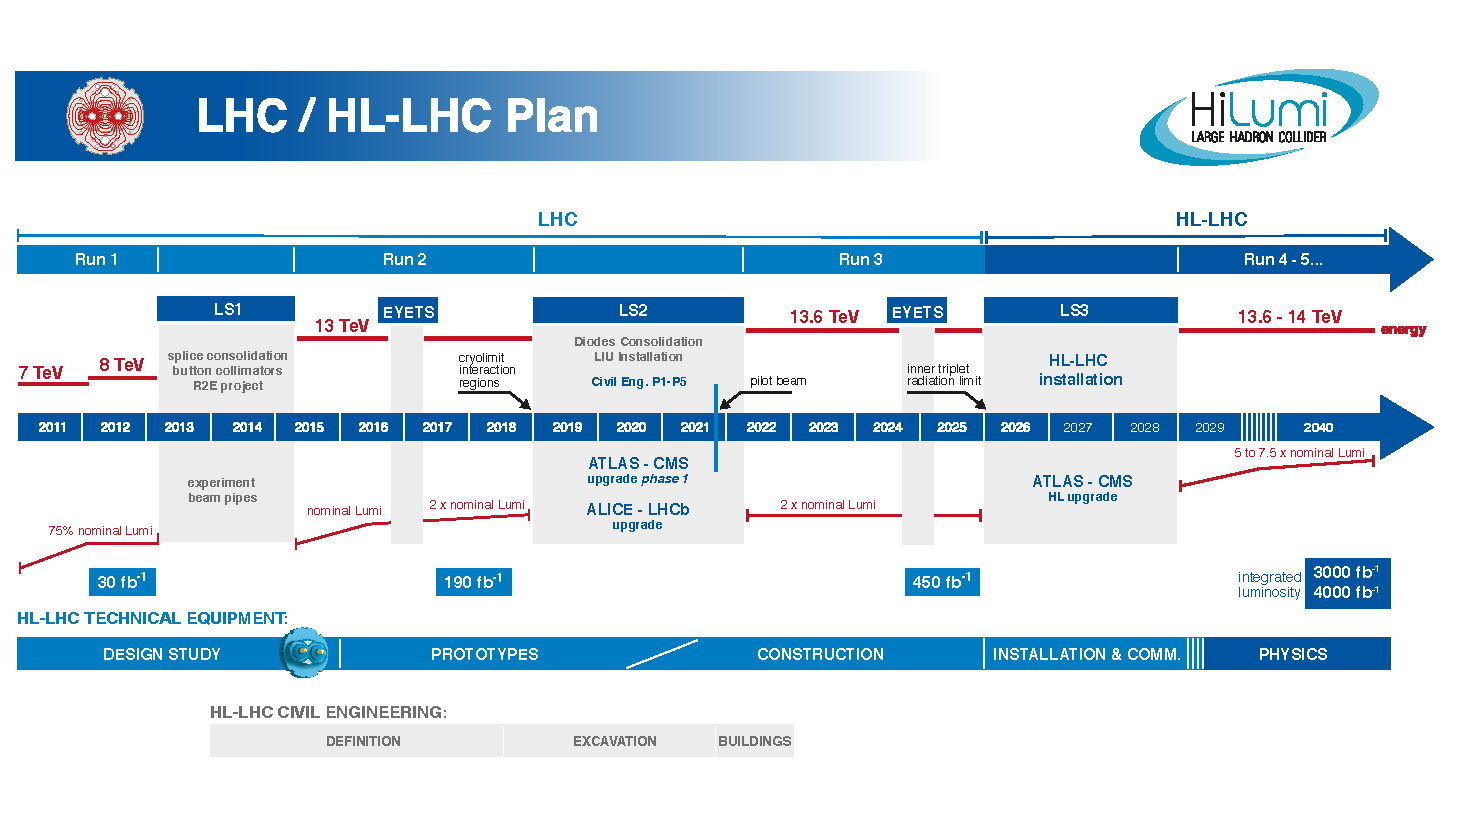
\includegraphics[width=1\linewidth]{fig//chap03-cms/LHC_schedule.pdf}
    \caption{Schedule of the LHC operations \cite{LS3Project}}
    \label{fig:lhc_schedule}
\end{figure}
\fi

\section{The Compact Muon Solenoid experiment}
The CMS experiment \cite{Chatrchyan2008TheLHC} is one of the two largest general-purpose detectors operating at CERN, located in Cessy(FR), 100 m underground at the LHC Point 5 (P5).\\
It is a cylindrical detector, 21.6 m long with a diameter of 14.6 m and a weight of 12500 tons, with coverage in pseudorapidity up to $|\eta|<3.0$\footnote{$\eta=-ln(\tan (\theta/2))$ where $\theta$ is the azimuthal angle in spherical coordinates} extended up to $|\eta|<5.0$ by the high forward Cherenkov calorimeter.\\
It consists of several subdetector layers, as shown in \Fig{fig:cms_exploded}: from inside out, the silicon tracker, the electromagnetic calorimeter (ECAL) and the hadronic calorimeter (HCAL) contained inside the solenoid magnet and the muon system embedded in the flux-return yoke outside the magnet.\\
The key features of the CMS detector are the strong solenoidal magnetic field of 3.8T that is designed to optimize the $p_T$ resolution of charged particles and a PbWO4 electromagnetic calorimeter that improves the $e/\gamma$ identification and resolution to maximize the sensitivity to the low mass $\gamma \gamma$ resonances.\\
These choices have some drawbacks: the PbWO4 crystals suffer radiation damage, becoming more and more opaque in time, and the solenoidal magnet constraint the size of the hadronic calorimeter to just 7 nuclear interaction lengths\footnote{The nuclear interaction length $\lambda$ of a certain material is the mean distance that hadronic particles travel in the material before interacting with a nucleus \label{fn:ncl}}, in contrast to the $10\lambda$ of the ATLAS experiment, affecting the jet energy resolution \cite{Spiropulu2012LHCsDETECTORS}.
\begin{figure}[h!]
    \centering
    \includegraphics[width=1\linewidth]{fig//chap03-cms/CMS_detector_white.pdf}
    \caption{Exploded view of the CMS detector \cite{Chatrchyan2008TheLHC}}
    \label{fig:cms_exploded}
\end{figure}

\subsection{Magnet}
The solenoid magnet \cite{Coroller1997TheReport} is the core element of the CMS experiment that has constrained the design of the rest of the detector.\\
The purpose of the magnet is to bend the tracks of charged particles, due to the Lorentz force, and allow us to measure the transverse momentum $p_T$ of the particle. The stronger the magnetic field, the better will be the $p_T$ resolution.\\
The magnet's coil is made up of multiple layers of superconducting niobium-titanium (NbTi) wires wound together that are cooled using liquid helium down to 4.7 K, allowing the coil to work in the superconductive regime.\\
The solenoidal geometry generates a quasi-uniform magnetic field inside the volume of the magnet of 3.8 T.
The solenoid is surrounded by the steel \emph{return yoke}, composed of five three-layered dodecagonal barrel wheels and three endcap disks at each end.  The yoke contributes to only 8\% of the central magnetic flux density \cite{Chatrchyan2010PreciseRays}. Its main role is to increase the field homogeneity inside the solenoid, closing the magnetic circuit and preventing magnetic leakage. It also hosts the muon system, embedding it in a 2 T magnetic field.

\begin{minipage}{\linewidth} 
    \vspace{0.5cm}
    %\hspace{-0.65cm}
    \begin{minipage}{0.65\linewidth}
        \centering
        \includegraphics[width=1\linewidth]{fig//chap03-cms/magnetic_field.png}
        \captionof{figure}{Field lines and magnitude of the magnetic field of the CMS solenoid magnet \cite{Chatrchyan2010PreciseRays}.}
        \label{fig:magnetic_field}
    \end{minipage}
    \hfill
    \begin{minipage}{0.3\linewidth}
        \centering
        \begin{tabular}{l|c}
            \hline
            Length &  12.5 m\\
            Diameter & 6 m\\
            Weight &  220 tons\\
            Solenoid $|B|$ &  3.8 T\\
            Yoke $|B|$ & 2 T\\
            \hline
        \end{tabular}
        \vspace{0.4cm}
        \captionof{table}{Specifics of the magnet}
    \end{minipage}
\end{minipage}

\subsection{Tracker}
The silicon tracker \cite{CastaldiPatriceSiegristJean-EudesAugustin1997TheReport,CMS_pixel_Phase1_2012} is the closest subdetector to the IP, covering the region $|\eta|<2.5$, and allows us to reconstruct the tracks of charged particles and their transverse momentum, measuring the curvature of the track caused by the magnet.
\begin{figure}[h!]
    \centering
    \includegraphics[width=0.73\linewidth]{fig//chap03-cms/CMS_tracker_Phase1_edit.pdf}
    \caption{Schematic view of a quarter of the CMS tracker in the $r-a$ plane. Pixel modules are shown in green, single-sided strip modules in red and double-sided strip modules in blue \cite{DPGResultsTRKTWiki}.}
    \label{fig:cms_tracker}
\end{figure}
\\
All the modules that compose the tracker are silicon semiconductor sensors and are divided into pixel modules that contain about 66 million pixel cells each with a size of $100 \times 150 \mu m^2$, and strips modules that contain strips of thickness from $80 \mu m$ to $205 \mu m$ and a length that increases with the pseudorapidity.\\
\\
The \emph{pixel tracker} \cite{Adam2021TheUpgrade} is the nearest component to the beam pipe. Its scope is not only limited to collecting the particle hits to reconstruct the tracks, but also to identifying and reconstructing the primary and secondary vertices. The vertex reconstruction is crucial to mitigate PU effects and to identify the decay of displaced particles, enhancing the b-tagging capabilities.
The high granularity of the pixel modules allows achieving these goals. Furthermore, being closest to the IP, the inner tracker has to be designed to be more radiation tolerant than the outer tracker.\\
The pixel tracker is composed of different parts:
\begin{itemize}
    \item \textbf{Barrel pixel (BPIX)}: 4 concentric layers of pixel modules.
    \item \textbf{Forward pixel (FPIX)}: 6 disks of pixel modules
    \begin{table}[h!]
        \centering
        \begin{tabular}{l|c|c|c|c}
            & Radius & z position & Number of & Dose \\
            & [mm]   &  [mm]    &  pixel modules & [Mrad]\\
            \hline
            BPIX & \multicolumn{4}{c}{ } \\
            \hline
            L1&29&-270 to +270&96& 100 \\
            L2&68&-270 to +270&224& 47\\
            L3&109&-270 to +270&352& 22\\
            L4&160&-270 to +270&512& 13 \\
            \hline
            FPIX & \multicolumn{4}{c}{ } \\
            \hline
            D1 inner&45–110&±338&88 & 21-106\\
            D1 outer&96–161&±309&136 & 13-28\\
            D2 inner&45–110&±413&88 & 21-106\\
            D2 outer&96–161&±384&136 & 13-28\\
            D3 inner&45–110&±508&88 & 21-106\\
            D3 outer&96–161&±479&136 & 13-28\\
        \end{tabular}
        \caption{Summary of average r, z positions, number of modules and dose for the four BPIX layers and
the six FPIX rings \cite{Adam2021TheUpgrade}.}
        \label{tab:pixel_tracker}
    \end{table}
\end{itemize}
The \emph{strip tracker} \cite{Friedl2001TheReadout} is composed of  $\sim 20000$ strip modules. Depending on the positions, the geometry of the sensors and the number of strips vary: In the barrel region, the sensors are rectangular, while the endcap sensors are trapezoidal.\\
Some modules are double-sided (DS) strip modules, \ie two single-sided (SS) strip modules mounted back to back with a strip inclination of 5.7° against each other (stereo configuration) to resolve the ambiguity on the z coordinate.


\begin{itemize}

    \item \textbf{Tracker inner barrel (TIB)}: 2 layers of DS + 2 layers of SS strip modules 
    \item \textbf{Tracker inner disk (TID)}: 2 layers of DS + 1 layers of SS strip modules 
    \item \textbf{Tracker outer barrel (TOB)}: 2 layers of DS + 4 layers of SS strip modules 
    \item \textbf{Tracker endcap (TEC)}: 3 layers of DS + 4 layers of SS strip modules 
\end{itemize}
\begin{table}[h!]
    \centering
    \fontsize{11.5pt}{11.5pt}\selectfont
    \begin{tabular}{l|c|c|c|c|c}
        Layer&Radius[mm]&Type&Modules&Pitch[mm]&Strips\\
        \hline
        TIB1&250&DS&336&80&768\\
        TIB2& 340& DS& 456& 80& 768\\
        TIB3&430&SS&552&120&512\\
        TIB4&520&SS&648&120&512\\
        TOB5&610&DS&504&122/183&768/512\\
        TOB6&696&DS&576&122/183&768/512\\
        TOB7&782&SS&648&183&512\\
        TOB8&868&SS&720&183&512\\
        TOB9&965&SS&792&122&768\\
        TOB10&1080&SS&888&122&768\\
        TID1&277&DS&144&81-112&768\\
        TID2&367&DS&144&113-143&768\\
        TID3&447&SS&240&124-158&512\\
        TEC1&277&DS&144&81-112&768\\
        TEC2&367&DS&288&113-143&768\\
        TEC3&447&SS&640&124-158&512\\
        TEC4&562&SS&1008&113-139&512\\
        TEC5&677&DS&720&126-156&768\\
        TEC6&891&SS&1008&163-205&512\\
        TEC7&991&SS&1440&140-172&512\\
    \end{tabular}
    \caption{Summary of average r, type, number of modules, pitch, and number of strips for the strip tracker \cite{Friedl2001TheReadout}.}
    \label{tab:strip_tracker}
\end{table}
The design of the tracker has to consider the multiple scattering, bremsstrahlung and photon conversion that can occur in the tracker itself and that can alter the trajectory and the measurement of the energy deposited in the calorimeter. This implies that the tracker should minimize the material budget without sacrificing the tracking capabilities.


\begin{figure}[H]
\centering
\begin{minipage}{\linewidth}
    \centering
\begin{minipage}{0.43\linewidth}
        \centering
        \includegraphics[width=\linewidth]{fig/chap03-cms/material_budget_lambda.png}
\end{minipage}
\hfill
\begin{minipage}{0.43\linewidth}
        \centering
        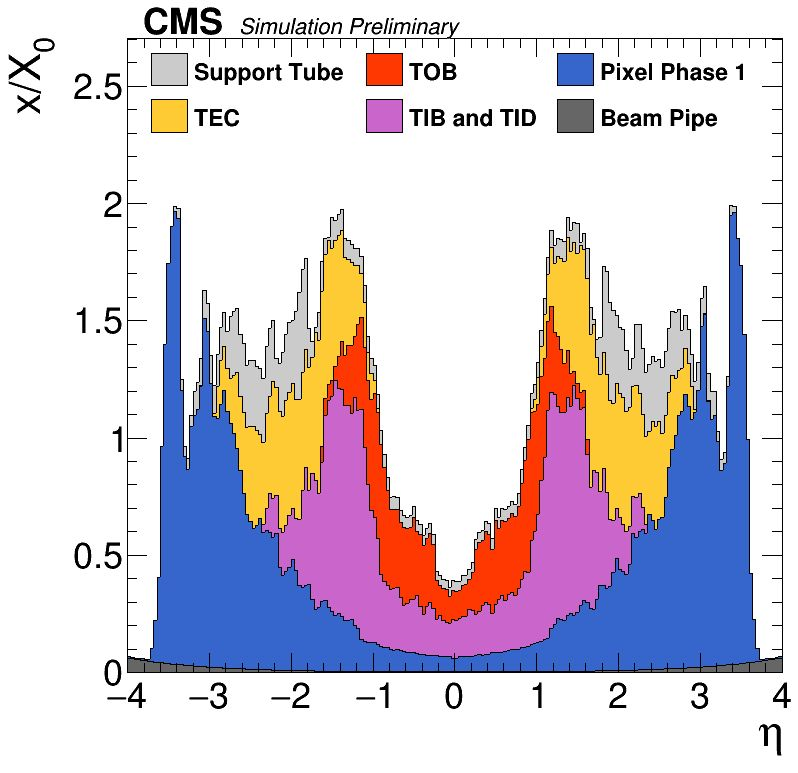
\includegraphics[width=\linewidth]{fig/chap03-cms/material_budget_X.png}
\end{minipage}
\caption[AAA]{Stacked histogram of the thickness of the subparts of the tracker traversed by a particle originated in the IP in function of $\eta$ ((left) in nuclear interaction length units\footnotemark[2], (right) in radiation length units)  \cite{TrackerMaterialBudgetplotsTWiki}.}
\end{minipage}
\end{figure}

%Footnote of the figure above
\footnotetext[2]{The radiation length $X_0$ of a given material is the length for which, for an electromagnetic particle that travels into the material, holds $E(z)=E_0 e^{-z/X_0}$ where $E(z)$ is the energy of the particle that is a function of the length traveled into the material and $E_0$ the initial energy.}


\subsection{Electromagnetic calorimeter}
The CMS electromagnetic calorimeter (ECAL) \cite{HoferETHZurichHansHofer1997TheReport,Biino2015TheProjections} is the subdetector dedicated to the identification and measurement of the energy of particles that interact primarily via the electromagnetic interaction.\\
One of the main goals of the CMS collaboration was the Higgs boson discovery and, to maximize the discovery sensitivity on the channel $H \to \gamma \gamma$, the ECAL should have met some requirements as high granularity and hermeticity, fast response ($\sim 25ns$), particle identification/isolation/energy at trigger level and linear response in a large energy range (5\GeV to 5\TeV).\\


To comply with these requirements, the ECAL was built using PbWO4 crystals: a high-density material ($\delta=8.28g/cm^3$) with a short radiation length ($X_0=0.85cm$) and a small Moliere radius\footnote{The Moliere radius $R_M$ is the mean radius of the cylinder that contains 90\% of the shower, which tends to disperse due to multiple scattering} ($R_M=2.19cm$).\\
The crystals emit optical light by scintillation in a short time (80\% of the light in 25ns, which is the time separation between two different bunch crossing) but, the light yields of only $\sim 100 \gamma/\MeV$ force the usage of an active photodetector and, due to the presence of the magnetic field, the silicon photomultipliers (SiPM) were the most logical choice.
The ECAL is made of a barrel that covers the $|\eta|<1.479$ region and two endcaps that cover the region $1.479<|\eta|<3.0$.

\begin{figure}[h!]
    \centering
    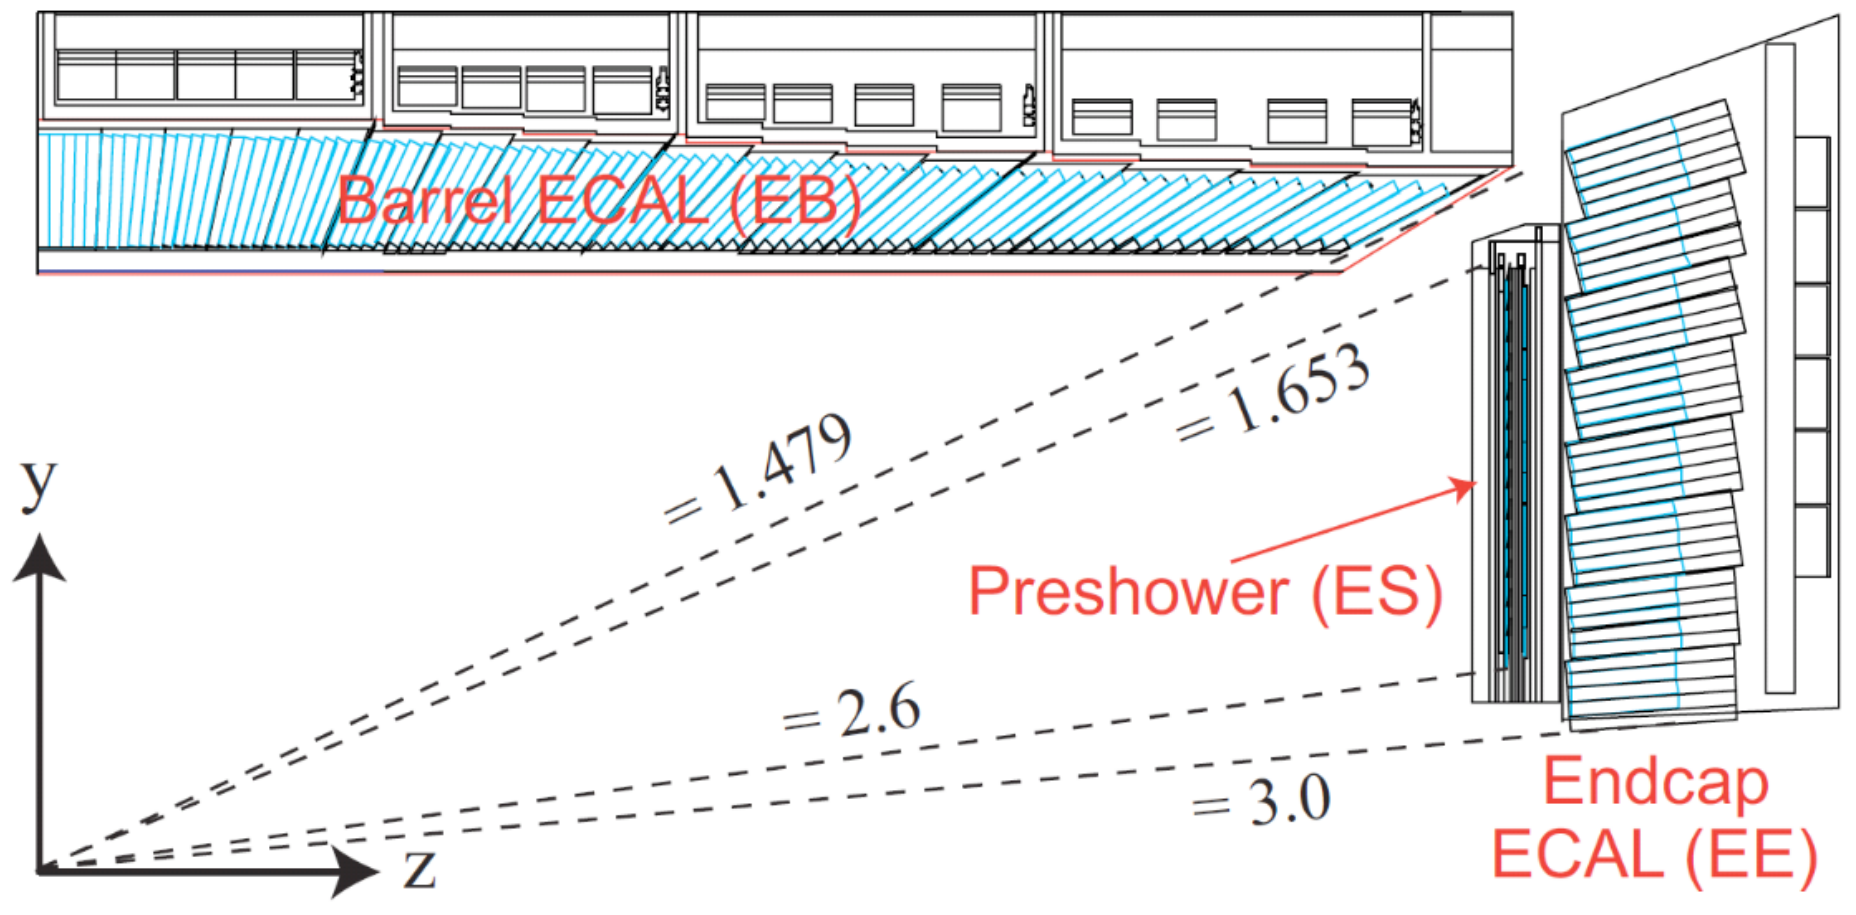
\includegraphics[width=0.7\linewidth]{fig/chap03-cms/ecal.png}
    \caption{Schematic view in the r-z plane of a quarter of the CMS ECAL \cite{Benaglia2014TheExamples}.}
    \label{fig:ecal}
\end{figure}
The ECAL endcaps are composed of 14648 crystals of size $3\times3\times22 cm^3 (\sim25X_0)$ and the ECAL barrel is composed of 61200 crystals of size $2.2\times2.2\times23 cm^3 (\sim26X_0)$. The crystals are not aligned to the IP to avoid cracks aligned with particle trajectories.\\
Furthermore, a pre-shower silicon detector made of 4288 strip modules is placed in front of the endcaps to improve the $\gamma-\pi^0$ separation\footnote{The $\pi^0$ decay $\pi^0 \to \gamma \gamma$ can cause the misidentification of a pion into a photon.}.
\\
\\
The energy resolution of the PbWO4 crystals measured with an electron beam without magnetic field and radiation damage was \cite{Adzic2007EnergyCalorimeter} 
\begin{equation}
    {\frac{\sigma_{E}}{E}}={\frac{2.8\%}{\sqrt{E[{\mathrm{GeV}}]}}}\oplus{\frac{0.127 \GeV}{E[{\mathrm{GeV}}]}}\oplus0.3\%
\end{equation}
where the first term is the stochastic term, the second is the noise term and the third is the constant term that contains the calibration errors and the leakage of the energy.\\
In the CMS detector, the ECAL energy resolution is worse mainly due to the presence of the tracker between the ECAL and the IP and due to the transparency variations induced by radiation damage and the aging of photomultipliers, but, during the Run1, the ECAL was able to achieve the $\sim1\%$ energy resolution for high-energy electrons \cite{Chatrchyan2013EnergyTeV}.\\
The radiation damage of PbWO4 crystals is constantly monitored by a laser system in various $\eta$ intervals as shown in \Fig{fig:ecal_rad_damage}.
\begin{figure}[h!]
    \centering
    \includegraphics[width=0.85\linewidth]{fig//chap03-cms/rad_damage.png}
    \caption{ECAL relative response to the laser monitoring system from 2011 to 2019 \cite{EcalDPGResultsCMSDPS2019005TWiki}.}
    \label{fig:ecal_rad_damage}
\end{figure}

\subsection{Hadronic calorimeter}
Hadrons usually don't deposit all their energy in the ECAL, especially neutral hadrons, therefore the ECAL is surrounded by the hadronic calorimeter HCAL that allows the measurements of the jets' energy and the missing energy.\\
The CMS HCAL \cite{Green1997TheReport,Anderson2012CMSCalorimeter} is divided into four subdetectors: the hadron barrel (HB), the hadron endcaps (HE), the hadron outer (HO), and the hadron forward (HF).\\
The HB is a sampling calorimeter made of brass absorbers and plastic scintillators that act as active material. The brass was chosen due to its short interaction length and because it is non-magnetic.\\
It covers the pseudorapidity region $|\eta|<1.3$ and it extends in a radius $1.77m<R<2.95m$. The barrel is divided into sections of size $(\Delta \eta, \Delta \phi)=0.087 \times 0.087$ and is composed of eight 50.5 mm thick and six 56.5 mm thick brass plates alternating with the scintillating tiles, that are connected through optical cables to SiPM sensors to collect and amplify the light.\\
The total thickness of the HB in nuclear interaction length units at $|\eta|=0$ is $5.82 \lambda_I$ that increases up to $10.6\lambda_I$ at $|\eta|=1.3$.\\
In addition to this, the ECAL barrel adds $\sim 1.1\lambda_I$ thickness of material.\\
\begin{figure}[h!]
    \centering
    \includegraphics[width=0.85\linewidth]{fig//chap03-cms/hcal.png}
    \caption{Schematic view in the r-z plane of a quarter of the CMS HCAL and depth segmentation after the Phase I update \cite{Anderson2012CMSCalorimeter}. }
    \label{fig:hcal}
\end{figure}
\\
Also the HE is a sampling calorimeter made of brass absorbers and plastic scintillating tiles. It is divided into 18 sectors in $\phi$ and into 14 sectors in $\eta$ (the size increases with $\eta$) and is placed 4006.5 mm from the interaction point. It covers the $1.3 < |\eta|<3.0$ region and including the ECAL endcaps, its length in interaction lengths units is $\sim10\lambda_I$\\
\\
The HO is placed outside the solenoid magnet, and its purpose is to catch the tails of the hadronic showers that are not contained by the HB. The HO is composed by five scintillator rings with a radius of 4.07 m that cover the region $|\eta|<1.26$. The central ring that covers the thinner HCAL region is equipped also with a 19.5 cm thick iron absorber and an additional scintillator, as shown in fig \Fig{fig:ecal_rad_damage}.\\
\\
The HF is a sampling calorimeter is located 11150 mm away from the interaction point and covers the region $3<|\eta|<5.2$. It is composed of 1.65 mm steel absorber plates and 0.6 mm thick quartz fibers that emit light by Cherenkov effect. It is also used for the online monitoring of luminosity.
\\
The combined energy resolution of the ECAL and the HCAL was measured using a pion beam from 2 \GeV to 350 \GeV \cite{Abdullin2008TheGeV/c}
\begin{equation}
    \frac{\sigma_E}{E}= \frac{84.7\%}{\sqrt{E}} \oplus 7.4 \%
\end{equation}
The energy resolution is mainly affected by the sampling fluctuations and the noise term is negligible.

\subsection{Muon system}
The CMS muon system \cite{Layter1997TheReport} is embedded in the iron return yoke and its scope is to collect muon hits that are used, in combination with information from the tracker, to enhance the identification of muons and momentum resolution of high-energy muons.
It is divided into five separate wheels in the barrel, containing four layers of detectors, and four independent endcaps for each side.

\begin{figure}[h!]
    \centering
    \includegraphics[width=0.85\linewidth]{fig//chap03-cms/muon_system.jpg}
    \caption{Schematic view in the $r-z$ plane of a quarter of the muon system \cite{Piccolo2011CMSPerformance}.}
    \label{fig:muon_system}
\end{figure}


Three different gaseous detector technologies are employed:
\begin{itemize}
    \item \textbf{Drift tubes chambers (DT)}: The 250 DT chambers are divided into five wheels and cover the region $|\eta|<1.2$. Each wheel is divided into 12 sectors covering $\Delta \phi=30º$ around the interaction point, and each sector is organized into four muon barrels (MB).
    Each chamber consists of 8 or 12 aluminum layers with up to 90 tubes.

    \item \textbf{Cathode strip chambers (CSC)}: CSCs consist of arrays of anode wires crossed with copper cathode strips within a gas volume. The 486 CSCs are organized in 4 layers, placed in the endcap disks, and extend the muon system coverage up to $0.8<|\eta|<2.4$

    
    \item \textbf{Resistive plate chambers (RPC)}: The RPCs are located both in the barrel and in the endcap region, up to $|\eta|<1.6$. RPCs consist of two charged parallel high resistive plastic plates filled with gas. The read-out is performed by aluminum strips separated from the graphite coating. The scope of the RPCs is to provide, in combination with the DTs and the CSCs, a fast signal to exploit for the muon trigger system.
\end{itemize}

\begin{figure}[H]
    \centering
    \begin{subfigure}[b]{.58\linewidth}
        
        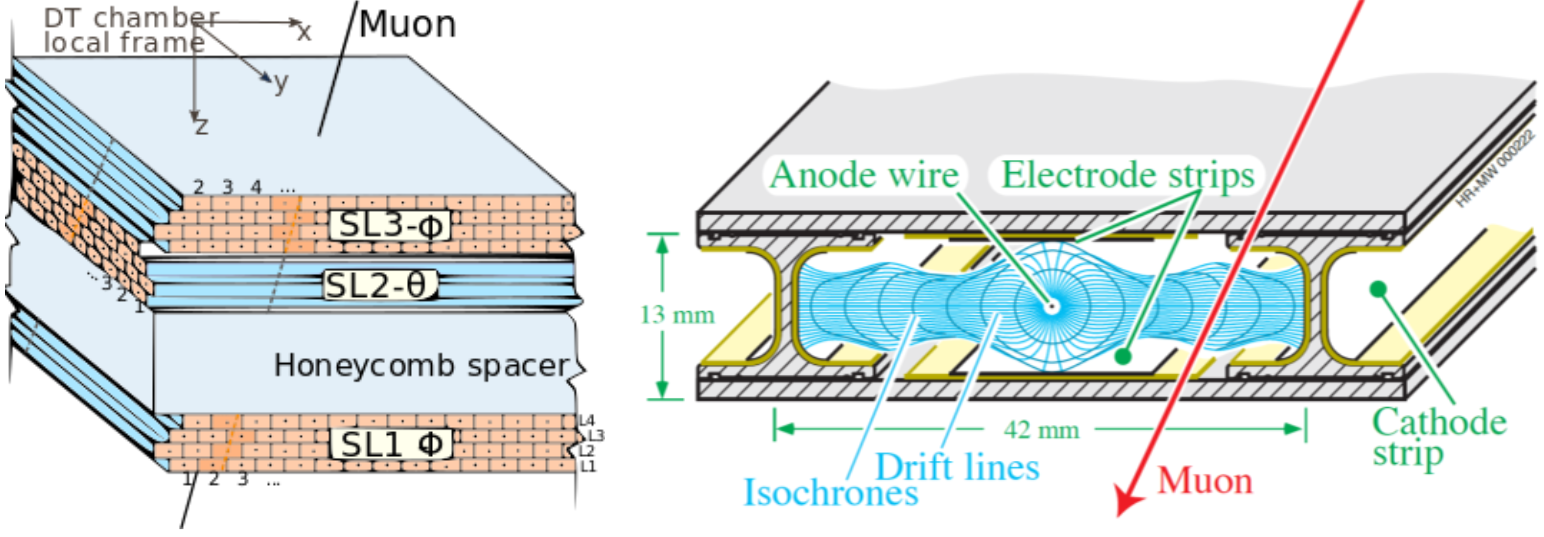
\includegraphics[width=\linewidth]{fig//chap03-cms/drift_tubes.png}
        \label{fig:drift_tubes}
        \caption{}
    \end{subfigure}
    \begin{subfigure}[b]{.41\linewidth}
        
        \includegraphics[width=1\linewidth]{fig//chap03-cms/rpc.png}
        \caption{}
        \label{fig:rpc}
    \end{subfigure}
    \begin{subfigure}[b]{0.7\linewidth}
        \centering
        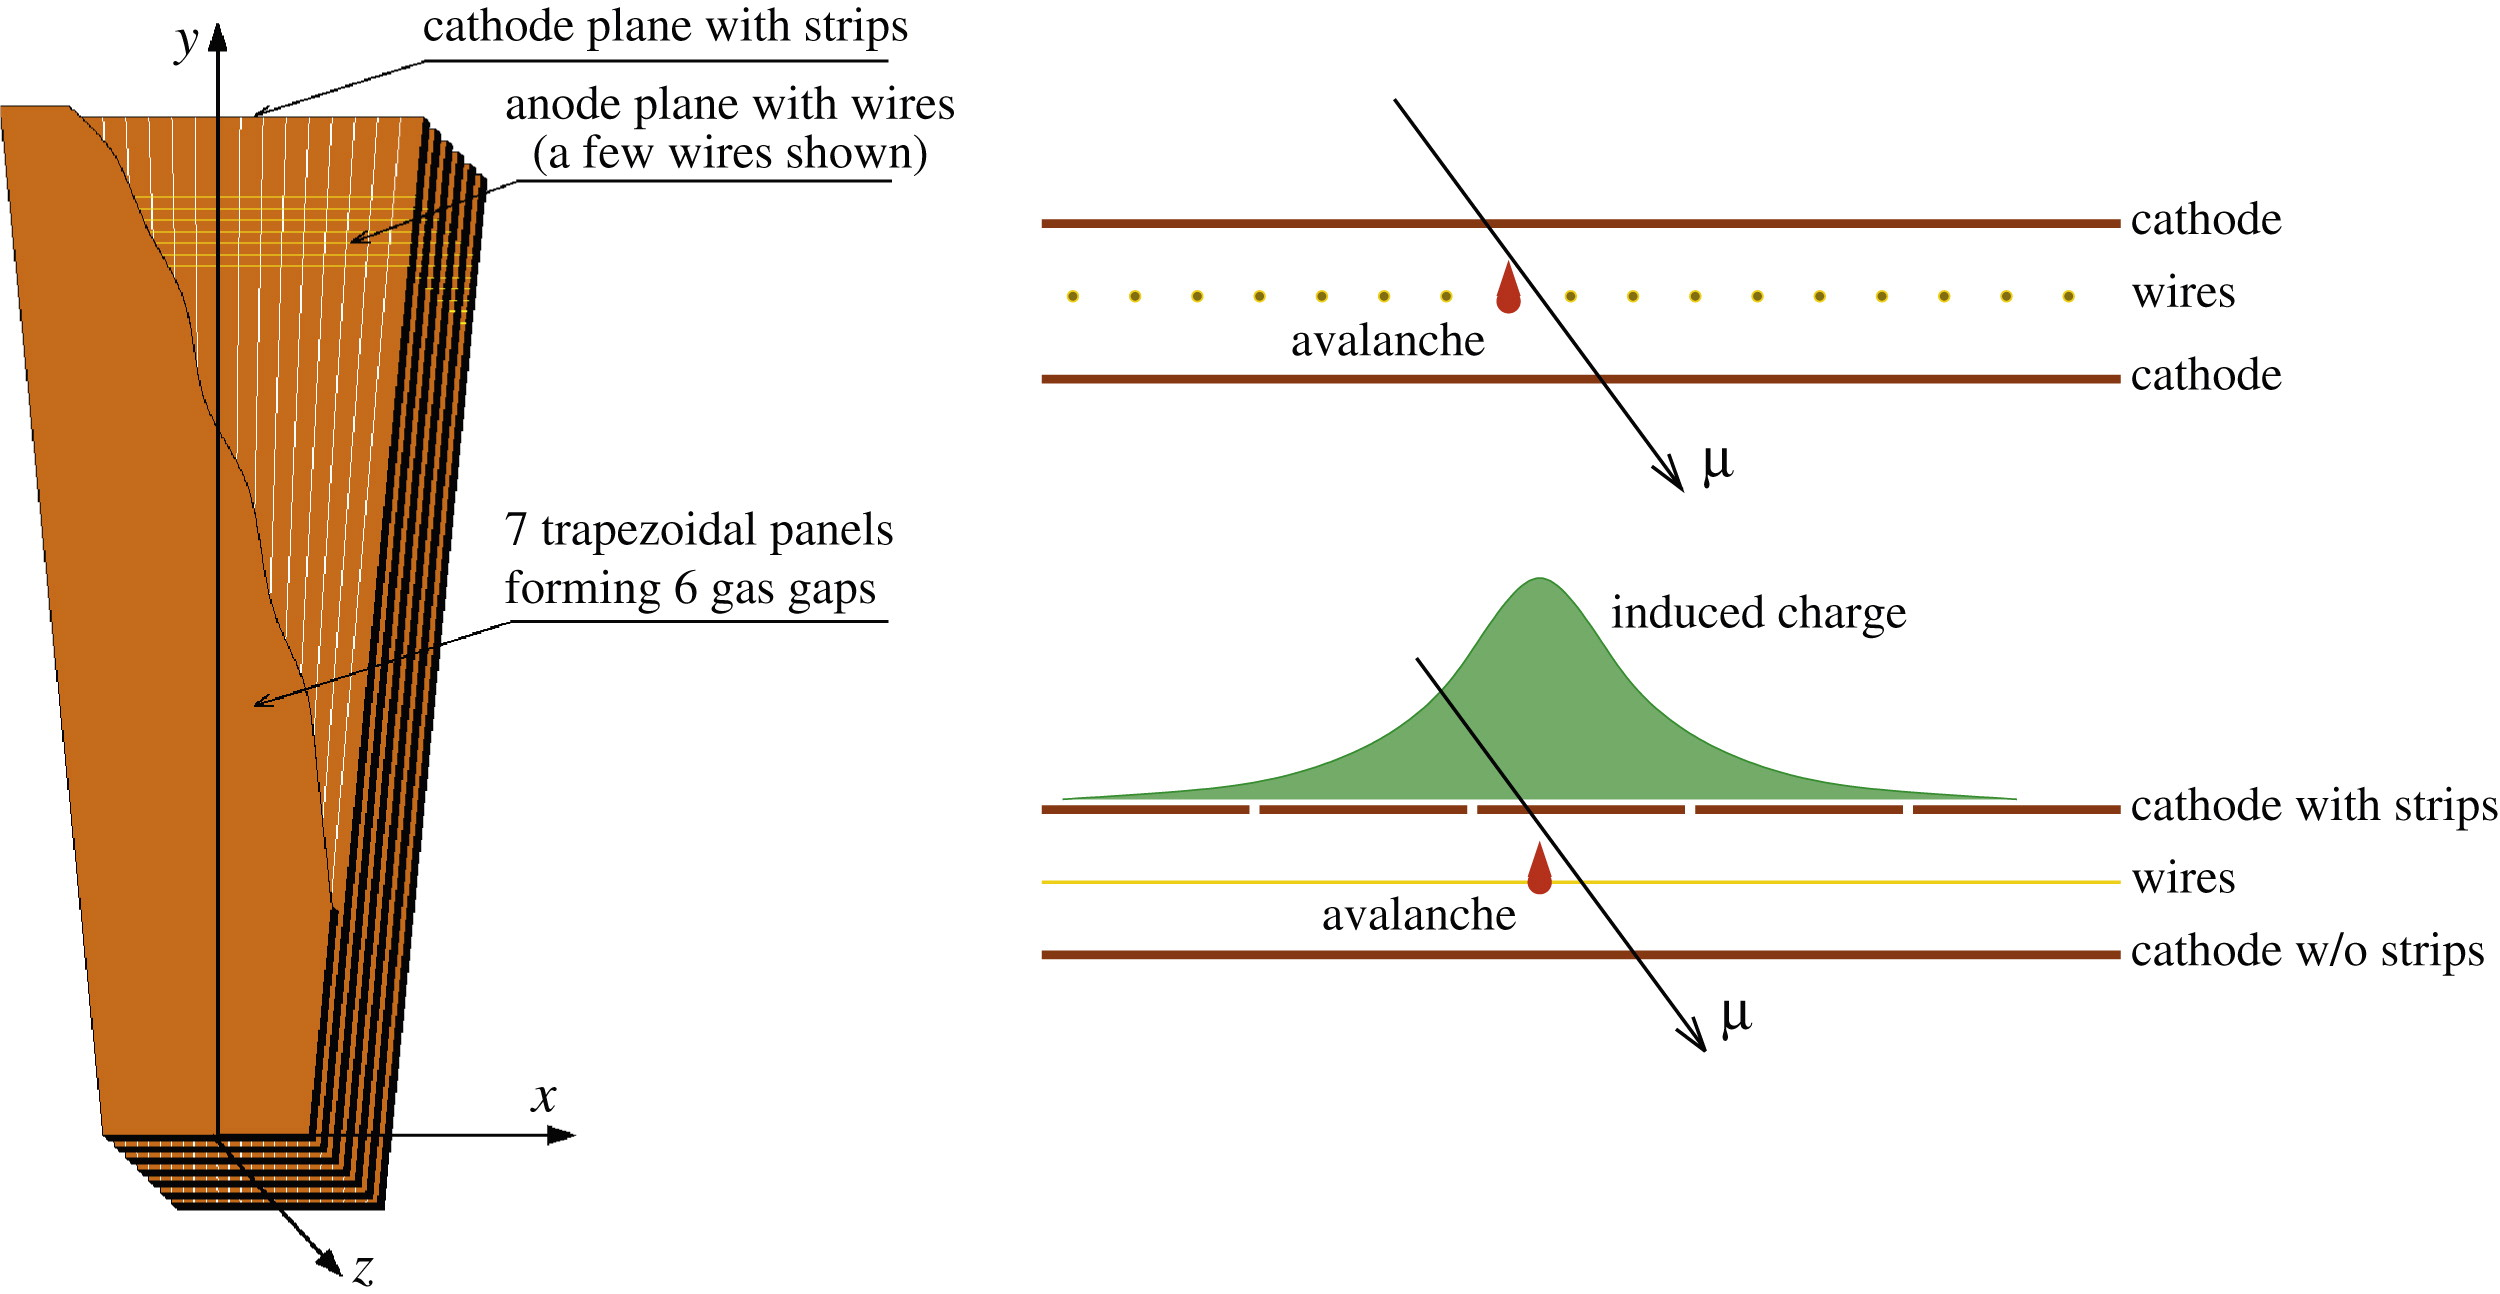
\includegraphics[width=1\linewidth]{fig//chap03-cms/csc.jpg}
        \caption{}
        \label{fig:csc}
    \end{subfigure}
    \caption{Schematics view of the (a) drift tubes chamber \cite{MuonExperiment}, (b) resistive plates \cite{EndcapReshufflingRpcTWiki}, (c) cathode strips chamber \cite{Acosta2008EfficiencyChambers}.}
    \label{fig:muons_technologies}
\end{figure}
    


\subsection{Trigger and data acquisition}
At LHC, bunch crossing occurs each 25ns. Considering the raw event size of 1 MB \cite{Franzoni2016DatasetAnalyses}, this would lead to a data throughput of  $\sim 1$ TB/s at the nominal luminosity, that, not only will saturate the bandwidth of the data acquisition system but also would make it impossible to save on tape all the recorded data.\\
The scope of the CMS trigger system is to select only the events relevant to the CMS physics program.
The trigger system is divided into the level 1 low-level trigger (L1) and the high-level trigger.\\
\\
The CMS L1 Trigger \cite{Musenich2000CMSSystems} operates as a hardware-based trigger system exploiting FPGA boards. It relies on custom algorithms that have to make decisions within $3.2 \mu s$, the maximum time that the raw data can occupy the buffers.\\
The L1 trigger collects raw data from the front-end electronics of the calorimeters and the muon system that converts the analog signals to digital.\\
The algorithms roughly estimate the energy deposit and the trajectory of the particles in the subdetectors to select EM, jet, and muon candidates. Thereafter, the information from the muon system and from the calorimeters are combined into the global trigger that chooses whether to discard the event or to pass it to the HLT trigger for further filtering.
The L1 trigger reduces the output rate from the bunch crossing rate of $40$MHz to $100$kHz.
\\
\begin{figure}[h!]
    \centering
    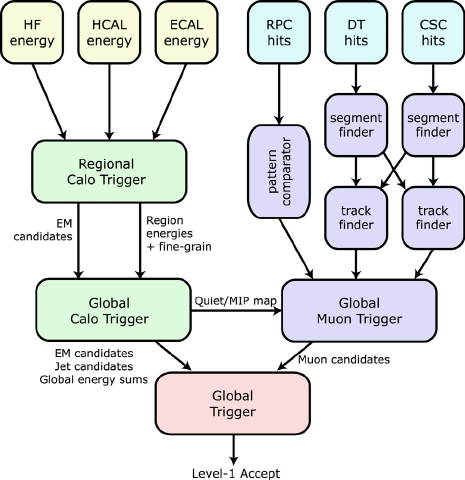
\includegraphics[width=0.6\linewidth]{fig/chap03-cms/L1.png}
    \caption{Architecture of the Level-1 Trigger \cite{Brooke2003HardwareTrigger}.}
    \label{fig:l1}
\end{figure}
\\
The HLT system \cite{Racz2002CMSTrigger} is a software-based trigger implemented on a computer farm composed of 16000 CPUs that decreases the output rate from the 100 kHz of the L1 trigger to 1 kHz. It employs the same algorithms used by the offline reconstruction but adapted to the timing constraint of the HLT trigger.
It has access to the full detector readout, and events are accepted or rejected as soon as there is enough information to decide. The raw data of the events that are accepted by the trigger are saved on tape and the events are reconstructed offline when the computing resources are available.

